% Компіляція: lualatex -shell-escape main.tex (двічі)
\documentclass[12pt,a4paper]{article}

\usepackage{fontspec}
\usepackage{polyglossia}
\setdefaultlanguage{ukrainian}
\setmainfont{NewComputerModern10}
\setsansfont{Noto Sans}
\setmonofont{Noto Sans Mono}[Scale=0.82]

\usepackage{amsmath,amssymb,array,booktabs,caption,enumitem,float,geometry,
  graphicx,longtable,microtype,needspace,titlesec,xcolor}
\geometry{left=2cm,right=2cm,top=2cm,bottom=2cm}
\setlength{\parindent}{1.25cm}
\setlength{\parskip}{0pt}
\linespread{1.08}
\titleformat{\section}{\normalfont\fontsize{14}{16}\selectfont\bfseries}
  {\thesection}{0.6em}{}
\titleformat{\subsection}{\normalfont\fontsize{12}{14}\selectfont\bfseries}
  {\thesubsection}{0.6em}{}
\titlespacing*{\section}{0pt}{1.4em}{0.65em}
\titlespacing*{\subsection}{0pt}{1.1em}{0.45em}
\captionsetup{font=small,labelfont=bf,labelsep=endash}
\captionsetup[table]{position=bottom,skip=5pt}

\usepackage[newfloat]{minted}
\SetupFloatingEnvironment{listing}{name=Лістинг}
\setminted{fontsize=\scriptsize,linenos,breaklines,breakanywhere,frame=single,
  framesep=2mm,bgcolor=gray!5,tabsize=4}

\usepackage{tikz}
\usetikzlibrary{arrows.meta,shapes.geometric,positioning,calc,fit}

\usepackage[unicode,colorlinks=true,linkcolor=black,urlcolor=blue,
  pdftitle={ІО-41, Давидчук А. М., Лабораторна робота №3.2},
  pdfauthor={Давидчук Артем Миколайович},
  pdfsubject={Монітори Java. Варіант 16}]{hyperref}

\newcommand{\studentName}{Давидчук А. М.}
\newcommand{\studentGroup}{ІО-41}
\newcommand{\recordBook}{4106}
\newcommand{\teacherName}{Корочкін О. В.}
\newcommand{\reportYear}{2026}

\begin{document}
\pagenumbering{gobble}
\begin{titlepage}
  \begin{center}
    
\includegraphics[width=0.7\textwidth]{../../../../../../templates/letterhead.png}
  \end{center}
  \begin{center}\large
    Національний технічний університет України\\
    «Київський політехнічний інститут імені Ігоря Сікорського»\\[1em]
    Факультет інформатики та обчислювальної техніки\\
    Кафедра обчислювальної техніки
  \end{center}
  \vfill
  \begin{center}
    \textbf{\LARGE Паралельні та розподілені обчислення}\\[2em]
    \textbf{\Large Лабораторна робота №3.2}\\[0.7em]
    \textbf{«Мова Java. Монітори»}
  \end{center}
  \vfill
  \begin{flushright}
    \begin{minipage}{0.48\textwidth}
      Виконав: студент 3 курсу ФІОТ,\\
      групи \studentGroup\\
      \textit{\studentName}\\
      Залікова книжка № \recordBook\\
      Варіант завдання: 16\\[1em]
      Перевірив: \textit{\teacherName}
    \end{minipage}
  \end{flushright}
  \vfill
  \begin{center}Київ --- \reportYear\end{center}
\end{titlepage}

\pagenumbering{arabic}

\section{Тема та мета роботи}
\noindent\textbf{Тема:} програмування для комп’ютерних систем зі спільною
пам’яттю з використанням моніторів мови Java.

\medskip
\noindent\textbf{Мета:} розробити паралельний алгоритм обчислення
векторно-матричного виразу; організувати взаємодію чотирьох потоків за
допомогою монітора Java; реалізувати взаємне виключення, умовне очікування
та сигналізацію методами \texttt{synchronized}, \texttt{wait()} і
\texttt{notifyAll()}; перевірити правильність програми та визначити її
прискорення на одному і чотирьох фізичних ядрах.

\section{Завдання}
За варіантом 16 необхідно обчислити
\begin{equation}
 A=p\bigl(\operatorname{sort}(dB+Z\cdot MM)\cdot(MX\cdot MT)\bigr)
   +(B\cdot Z)Z.
 \label{eq:task}
\end{equation}
Тут $A,B,Z$ --- вектори довжини $N$; $MM,MX,MT$ --- квадратні матриці
порядку $N$; $d,p$ --- скаляри; $B\cdot Z$ --- скалярний добуток
векторів; $\operatorname{sort}$ --- сортування вектора за зростанням.
Кількість потоків $P=4$. Розподіл введення і виведення наведено в
табл.~\ref{tab:io}.

\begin{table}[H]
\centering\renewcommand{\arraystretch}{1.2}
\begin{tabular}{|c|c|c|}\hline
\textbf{Потік} & \textbf{Введення} & \textbf{Виведення}\\\hline
$T_1$ & $MM,B,MX$ & ---\\\hline
$T_2$ & --- & ---\\\hline
$T_3$ & $p$ & ---\\\hline
$T_4$ & $Z,MT,d$ & $A$\\\hline
\end{tabular}
\caption{Розподіл операцій введення і виведення для варіанта 16}
\label{tab:io}
\end{table}

\section{ВИКОНАННЯ ЛР}

\subsection{Етап 1. Розроблення паралельного математичного алгоритму}
Позначимо
\begin{equation}
 U=dB+Z\cdot MM,\qquad MC=MX\cdot MT,\qquad b=B\cdot Z,
 \qquad S=\operatorname{sort}(U).
\end{equation}
Тоді заданий вираз набуває вигляду
\begin{equation}
 A=p(S\cdot MC)+bZ.
\end{equation}

Для потоку з номером $t\in\{0,1,2,3\}$ визначимо
\begin{equation}
 a_t=\left\lfloor\frac{tN}{4}\right\rfloor,\qquad
 e_t=\left\lfloor\frac{(t+1)N}{4}\right\rfloor,\qquad
 J_t=\{a_t,\ldots,e_t-1\}.
 \label{eq:ranges}
\end{equation}
Діапазони не перетинаються й охоплюють усі індекси навіть тоді, коли
$N$ не кратне чотирьом. Потік $T_{t+1}$ записує елементи векторів і
стовпці матриць лише з індексами $j\in J_t$.

Паралельний математичний алгоритм:
\begin{align}
1.\quad &U_H=dB_H+Z\cdot MM_H; \label{eq:u-h}\\
2.\quad &MC_H=MX\cdot MT_H; \label{eq:mc-h}\\
3.\quad &b_i=B_H\cdot Z_H,\qquad i=1,2,3,4; \label{eq:bi}\\
4.\quad &b=b+b_i,\qquad b_{\mathrm{поч}}=0; \label{eq:b-reduction}\\
5.\quad &S=\operatorname{sort}(U); \label{eq:sort}\\
6.\quad &A_H=p(S\cdot MC_H)+bZ_H. \label{eq:a-h}
\end{align}
На кроці~\eqref{eq:b-reduction} кожен потік виконує повну операцію
читання, додавання та запис спільного $b$ у синхронізованому методі
монітора. Сортування на кроці~\eqref{eq:sort} є глобальним: просте
об’єднання чотирьох окремо відсортованих частин не гарантувало б
відсортованості всього $U$. Тому після готовності всіх частин $U$ потік
$T_4$ виконує \texttt{Arrays.sort(U)} і сигналізує іншим потокам.

В елементній формі для $j\in J_t$:
\begin{align}
 U_j &= dB_j+\sum_{k=0}^{N-1}Z_kMM_{k,j},\\
 MC_{i,j} &= \sum_{k=0}^{N-1}MX_{i,k}MT_{k,j},
 &&i=0,\ldots,N-1,\\
 b_t &= \sum_{k=a_t}^{e_t-1}B_kZ_k,\\
 A_j &= p\sum_{k=0}^{N-1}S_kMC_{k,j}+bZ_j.
\end{align}

\subsubsection*{Спільні ресурси}
Спільними є вхідні дані $B,Z,MM,MX,MT,d,p$, проміжні результати
$U,MC,S$, кінцевий вектор $A$, скаляр $b$, консоль і об’єкт
\texttt{Scanner}. Після завершення введення вхідні дані лише читаються.
Різні потоки записують неперетинні частини $U$, $MC$ та $A$, тому ці
операції не потребують взаємного виключення. Скаляр $b$ читається і
змінюється всіма потоками, тому є справжнім спільним ресурсом.

\subsection{Етап 2. Розроблення алгоритмів потоків}
Позначення $S_{j,k}$ означає сигнал задачі $T_j$, а $W_{j,k}$ ---
очікування події в задачі $T_j$; $k$ є номером взаємодії. У програмі
попарні логічні сигнали об’єднані лічильниками та прапорцем монітора.
Один виклик \texttt{notifyAll()} сповіщає всі задачі, але кожна з них
продовжує роботу лише після повторної перевірки своєї умови в циклі
\texttt{while}.

\begin{longtable}{|p{0.65cm}|p{10.6cm}|p{3.0cm}|}
\hline
\textbf{№}&\textbf{Алгоритм потоку $T_1$}&\textbf{Точка / КД}\\\hline
1&У моніторі ввести $MM,B,MX$.&КД $M_{in}$\\\hline
2&Сигналізувати про завершення своєї операції введення.&$S_{2,1},S_{3,1},S_{4,1}$\\\hline
3&Чекати завершення введення у $T_3,T_4$.&$W_{3,1},W_{4,1}$\\\hline
4&Обчислити $U_{J_0}$ за формулою~\eqref{eq:u-h}.&---\\\hline
5&Обчислити стовпці $MC_{:,J_0}$ за формулою~\eqref{eq:mc-h}.&---\\\hline
6&Обчислити $b_1=B_{J_0}\cdot Z_{J_0}$.&---\\\hline
7&У моніторі виконати $b=b+b_1$ та сигналізувати готовність проміжних результатів.&КД $M_b$; $S_{2,2},S_{3,2},S_{4,2}$\\\hline
8&Чекати готовності проміжних результатів інших потоків; скопіювати $b$.&$W_{2,2},W_{3,2},W_{4,2}$\\\hline
9&Чекати завершення глобального сортування в $T_4$.&$W_{4,3}$\\\hline
10&Обчислити $A_{J_0}$ за формулою~\eqref{eq:a-h}.&---\\\hline
11&Сигналізувати $T_4$ про готовність $A_{J_0}$.&$S_{4,4}$\\\hline
\end{longtable}

\begin{longtable}{|p{0.65cm}|p{10.6cm}|p{3.0cm}|}
\hline
\textbf{№}&\textbf{Алгоритм потоку $T_2$}&\textbf{Точка / КД}\\\hline
1&Чекати завершення введення у $T_1,T_3,T_4$.&$W_{1,1},W_{3,1},W_{4,1}$\\\hline
2&Обчислити $U_{J_1}$ за формулою~\eqref{eq:u-h}.&---\\\hline
3&Обчислити стовпці $MC_{:,J_1}$ за формулою~\eqref{eq:mc-h}.&---\\\hline
4&Обчислити $b_2=B_{J_1}\cdot Z_{J_1}$.&---\\\hline
5&У моніторі виконати $b=b+b_2$ та сигналізувати готовність проміжних результатів.&КД $M_b$; $S_{1,2},S_{3,2},S_{4,2}$\\\hline
6&Чекати готовності проміжних результатів інших потоків; скопіювати $b$.&$W_{1,2},W_{3,2},W_{4,2}$\\\hline
7&Чекати завершення глобального сортування в $T_4$.&$W_{4,3}$\\\hline
8&Обчислити $A_{J_1}$ за формулою~\eqref{eq:a-h}.&---\\\hline
9&Сигналізувати $T_4$ про готовність $A_{J_1}$.&$S_{4,4}$\\\hline
\end{longtable}

\begin{longtable}{|p{0.65cm}|p{10.6cm}|p{3.0cm}|}
\hline
\textbf{№}&\textbf{Алгоритм потоку $T_3$}&\textbf{Точка / КД}\\\hline
1&У моніторі ввести $p$.&КД $M_{in}$\\\hline
2&Сигналізувати про завершення своєї операції введення.&$S_{1,1},S_{2,1},S_{4,1}$\\\hline
3&Чекати завершення введення у $T_1,T_4$.&$W_{1,1},W_{4,1}$\\\hline
4&Обчислити $U_{J_2}$ за формулою~\eqref{eq:u-h}.&---\\\hline
5&Обчислити стовпці $MC_{:,J_2}$ за формулою~\eqref{eq:mc-h}.&---\\\hline
6&Обчислити $b_3=B_{J_2}\cdot Z_{J_2}$.&---\\\hline
7&У моніторі виконати $b=b+b_3$ та сигналізувати готовність проміжних результатів.&КД $M_b$; $S_{1,2},S_{2,2},S_{4,2}$\\\hline
8&Чекати готовності проміжних результатів інших потоків; скопіювати $b$.&$W_{1,2},W_{2,2},W_{4,2}$\\\hline
9&Чекати завершення глобального сортування в $T_4$.&$W_{4,3}$\\\hline
10&Обчислити $A_{J_2}$ за формулою~\eqref{eq:a-h}.&---\\\hline
11&Сигналізувати $T_4$ про готовність $A_{J_2}$.&$S_{4,4}$\\\hline
\end{longtable}

\begin{longtable}{|p{0.65cm}|p{10.6cm}|p{3.0cm}|}
\hline
\textbf{№}&\textbf{Алгоритм потоку $T_4$}&\textbf{Точка / КД}\\\hline
1&У моніторі ввести $Z,MT,d$.&КД $M_{in}$\\\hline
2&Сигналізувати про завершення своєї операції введення.&$S_{1,1},S_{2,1},S_{3,1}$\\\hline
3&Чекати завершення введення у $T_1,T_3$.&$W_{1,1},W_{3,1}$\\\hline
4&Обчислити $U_{J_3}$ за формулою~\eqref{eq:u-h}.&---\\\hline
5&Обчислити стовпці $MC_{:,J_3}$ за формулою~\eqref{eq:mc-h}.&---\\\hline
6&Обчислити $b_4=B_{J_3}\cdot Z_{J_3}$.&---\\\hline
7&У моніторі виконати $b=b+b_4$ та сигналізувати готовність проміжних результатів.&КД $M_b$; $S_{1,2},S_{2,2},S_{3,2}$\\\hline
8&Чекати готовності проміжних результатів інших потоків; скопіювати $b$.&$W_{1,2},W_{2,2},W_{3,2}$\\\hline
9&Виконати $S=\operatorname{sort}(U)$; сигналізувати $T_1,T_2,T_3$.&$S_{1,3},S_{2,3},S_{3,3}$\\\hline
10&Обчислити $A_{J_3}$ за формулою~\eqref{eq:a-h}.&---\\\hline
11&Чекати готовності $A_{J_0},A_{J_1},A_{J_2}$.&$W_{1,4},W_{2,4},W_{3,4}$\\\hline
12&У моніторі вивести $A$.&КД $M_{out}$\\\hline
\end{longtable}

\subsection{Етап 3. Визначення засобів взаємодії та структурна схема}
Взаємодію реалізує один спільний екземпляр класу \texttt{Monitor}, посилання
на який передається всім чотирьом потокам. Кожний його метод
\texttt{synchronized}, тому одночасно всередині монітора перебуває лише один
потік. Метод \texttt{wait()} звільняє lock монітора під час очікування, а
\texttt{notifyAll()} пробуджує всі задачі, які повторно перевіряють умови.

\begin{table}[H]
\centering\footnotesize\renewcommand{\arraystretch}{1.15}
\begin{tabular}{|p{4.9cm}|p{9.5cm}|}\hline
\textbf{Поле або метод монітора}&\textbf{Призначення}\\\hline
\texttt{inputT1/T3/T4()}&Взаємне виключення для консолі та спільного \texttt{Scanner}; введення одного потоку не перемішується з введенням іншого.\\\hline
\texttt{inputCount}, \texttt{signalInput()}, \texttt{waitInput()}&Очікування завершення трьох операцій введення перед початком обчислень.\\\hline
\texttt{b}, \texttt{addPartialBAndSignal()}&Критична ділянка $b=b+b_i$ та реєстрація готовності $U_{J_t}$, $MC_{:,J_t}$, $b_i$.\\\hline
\texttt{intermediateCount}, \texttt{waitIntermediateAndCopyB()}&Очікування чотирьох проміжних результатів і копіювання остаточного $b$ у локальну змінну.\\\hline
\texttt{sortFinished}, \texttt{signalSortFinished()}, \texttt{waitSortFinished()}&Сигнал і очікування завершення глобального сортування $U$.\\\hline
\texttt{calculationCount}, \texttt{signalCalculationFinished()}, \texttt{waitOtherCalculations()}&Три сигнали від $T_1,T_2,T_3$ та їх очікування в $T_4$ перед виведенням $A$.\\\hline
\texttt{printResult()}&Взаємне виключення під час виведення результату.\\\hline
\end{tabular}
\caption{Засоби взаємодії, реалізовані монітором}
\label{tab:monitor}
\end{table}

\begin{figure}[H]
\centering
\resizebox{\textwidth}{!}{\begin{tikzpicture}[
  font=\small,
  task/.style={draw,fill=yellow!12,trapezium,trapezium left angle=82,
    trapezium right angle=98,minimum width=3.2cm,minimum height=1.45cm,align=center},
  monitor/.style={draw,fill=blue!7,minimum width=6.2cm,minimum height=5.6cm,align=center},
  method/.style={draw,rounded corners,fill=green!12,minimum width=3.7cm,
    minimum height=0.55cm,align=center,font=\scriptsize},
  arrow/.style={-Latex,thick},
  both/.style={<->,>=Latex,thick}
]
  \node[task] (t1) at (-7.0, 2.4) {$T_1$\\введення $MM,B,MX$\\обчислення $U_{J_0},MC_{:,J_0},b_1,A_{J_0}$};
  \node[task] (t2) at (-7.0,-2.4) {$T_2$\\без введення\\обчислення $U_{J_1},MC_{:,J_1},b_2,A_{J_1}$};
  \node[task] (t3) at ( 7.0, 2.4) {$T_3$\\введення $p$\\обчислення $U_{J_2},MC_{:,J_2},b_3,A_{J_2}$};
  \node[task] (t4) at ( 7.0,-2.4) {$T_4$\\введення $Z,MT,d$; $\operatorname{sort}(U)$\\обчислення $U_{J_3},MC_{:,J_3},b_4,A_{J_3}$\\виведення $A$};

  \node[monitor] (mon) at (0,0) {};
  \node[font=\bfseries] at (0,2.45) {Монітор \texttt{Monitor}};
  \node[align=center,font=\scriptsize] at (0,1.85)
    {$inputCount=0$, $intermediateCount=0$,\\$sortFinished=false$, $calculationCount=0$, $b=0$};

  \node[method] (input) at (0,1.05) {\texttt{inputT1(), inputT3(), inputT4()}};
  \node[method] (wi) at (0,0.35) {\texttt{signalInput(), waitInput()}};
  \node[method] (bi) at (0,-0.35) {\texttt{addPartialBAndSignal(),}\\\texttt{waitIntermediateAndCopyB()}};
  \node[method] (sort) at (0,-1.15) {\texttt{signalSortFinished(),}\\\texttt{waitSortFinished()}};
  \node[method] (out) at (0,-1.95) {\texttt{signalCalculationFinished(),}\\\texttt{waitOtherCalculations(), printResult()}};

  \draw[both] (t1.east) -- (mon.west |- t1.east);
  \draw[both] (t2.east) -- (mon.west |- t2.east);
  \draw[both] (t3.west) -- (mon.east |- t3.west);
  \draw[both] (t4.west) -- (mon.east |- t4.west);

  \node[draw,fit=(t1)(t2)(t3)(t4)(mon),inner sep=0.35cm,
    label={[font=\bfseries]above:Спільна пам’ять і монітор взаємодії}] {};
\end{tikzpicture}
}
\caption{Структурна схема взаємодії потоків через монітор}
\label{fig:interaction}
\end{figure}

На рис.~\ref{fig:interaction} монітор показано окремим класом із власним
станом і методами, як у зразку структурної схеми для ЛР3. Стрілки
означають виклики методів монітора потоками та повернення з них. Довгі
матричні обчислення й сортування виконуються поза синхронізованими
методами, тому lock монітора не серіалізує основне навантаження.

\subsection{Етап 4. Розроблення програми}
Програму написано мовою Java. Клас \texttt{Main} створює спільні об’єкти
\texttt{Data} і \texttt{Monitor}, чотири потоки та очікує їх завершення
методом \texttt{join()}. Клас \texttt{Data} містить вхідні, проміжні й
результуючі масиви та математичні операції. \texttt{Worker} містить
спільну послідовність обчислювальних дій, а \texttt{T1}--\texttt{T4}
задають введення, очікування, сигналізацію та виведення відповідно до
табл.~\ref{tab:io}.

Вектори й матриці зберігаються в масивах типу \texttt{long}. Для введення
кожного вектора або матриці задається одне число, яким заповнюються всі
елементи. Час фіксується після завершення всього введення і до готовності
всіх частин $A$; друк результату до вимірювання не входить.

\subsection{Етап 5. Тестування програми}
Контрольний тест виконано при $N=4$, коли всі елементи вхідних векторів і
матриць, а також $p$ і $d$, дорівнюють одиниці. Тоді
\begin{align*}
 U_j&=1+4=5, & MC_{i,j}&=4, & b&=4,\\
 (S\cdot MC)_j&=4\cdot5\cdot4=80, & A_j&=80+4=84.
\end{align*}
Програма отримала $A=[84,84,84,84]$, що збігається з теоретичним
результатом. Додатково перевірено $N=5$: отримано п’ять значень 155, що
підтверджує коректний розподіл індексів для $N$, не кратного чотирьом.

Швидкодію досліджено при $N=1000$ і одиничних вхідних даних. Для одного
ядра використано \texttt{taskset -c 0}, для чотирьох різних фізичних ядер
--- \texttt{taskset -c 0,2,4,6}. Виконано по три окремі запуски; за
підсумковий час узято медіану.

\begin{table}[H]
\centering\renewcommand{\arraystretch}{1.15}
\begin{tabular}{|c|c|c|c|}\hline
\textbf{Режим}&\textbf{Запуск 1, с}&\textbf{Запуск 2, с}&\textbf{Запуск 3, с}\\\hline
1 фізичне ядро&1,581894&1,358938&1,352052\\\hline
4 фізичні ядра&0,414366&0,336436&0,350704\\\hline
\end{tabular}
\caption{Час обчислення при $N=1000$}
\label{tab:time}
\end{table}

Медіанні значення: $t_1=1{,}358938$ с, $t_4=0{,}350704$ с. Коефіцієнт
прискорення та ефективність:
\begin{equation}
 K_p=\frac{t_1}{t_4}=\frac{1{,}358938}{0{,}350704}=3{,}875,
 \qquad E_p=\frac{K_p}{4}\cdot100\%=96{,}9\%.
\end{equation}

На рис.~\ref{fig:cpu-one} наведено контроль завантаження під час запуску
з прив’язкою до одного ядра: процесор $C0$ завантажений на 100\%, тоді як
інші ядра виконують лише фонові системні задачі. На
рис.~\ref{fig:cpu-four} показано запуск із прив’язкою до чотирьох фізичних
ядер: одночасно повністю завантажені $C0$, $C2$, $C4$ і $C6$.
\begin{figure}[H]
\centering
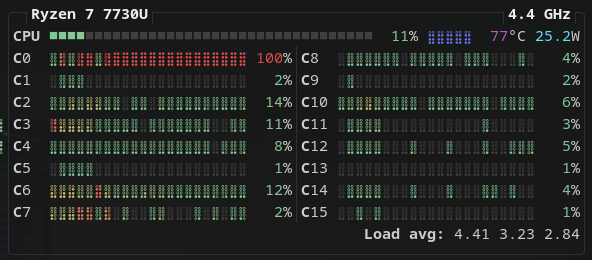
\includegraphics[width=0.83\textwidth]{image1.png}
\caption{Завантаження процесора під час запуску на одному ядрі}
\label{fig:cpu-one}
\end{figure}

\begin{figure}[H]
\centering
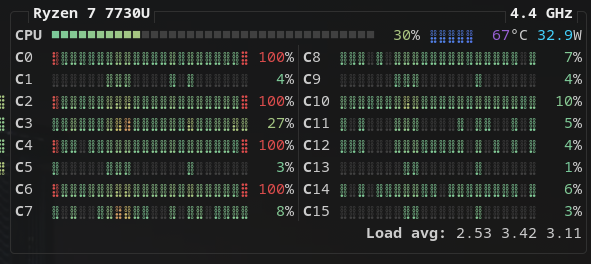
\includegraphics[width=0.83\textwidth]{image2.png}
\caption{Завантаження процесора під час запуску на чотирьох фізичних ядрах}
\label{fig:cpu-four}
\end{figure}

\section{Висновки}
\begin{enumerate}[leftmargin=*,itemsep=0.35em]
\item Розроблено паралельний математичний алгоритм виразу варіанта 16.
Роботу розподілено за частинами векторів і стовпцями матриць; визначено
спільний скаляр $b$ та залежність від глобально відсортованого $U$.
\item Розроблено алгоритми $T_1$--$T_4$ за формулами етапу 1 із
критичними ділянками та точками сигналізації й очікування. Довгі
обчислення виконуються поза монітором, а потоки записують неперетинні
частини $U$, $MC$ та $A$.
\item Визначено засоби взаємодії: один спільний Java-монітор,
синхронізовані методи, лічильники завершення фаз, прапорець готовності
сортування, \texttt{wait()} та \texttt{notifyAll()}. Побудовано структурну
схему класу-монітора та його зв’язків із чотирма потоками.
\item Розроблено й налагоджено програму мовою Java. Контрольні тести для
$N=4$ і $N=5$ підтвердили правильність результату та розподілу індексів.
\item Проведено тестування при $N=1000$. Медіанний час зменшився з
1,358938 с на одному ядрі до 0,350704 с на чотирьох фізичних ядрах;
$K_p=3{,}875$, ефективність --- 96,9\%. Відхилення від теоретичного
прискорення 4 пояснюється глобальним сортуванням, синхронізацією фаз і
службовими витратами JVM.
\end{enumerate}

\clearpage
\appendix
\section{Лістинг програми}
\subsection{Головний клас Main.java}
\inputminted{java}{../src/Main.java}
\subsection{Клас даних Data.java}
\inputminted{java}{../src/Data.java}
\subsection{Клас-монітор Monitor.java}
\inputminted{java}{../src/Monitor.java}
\subsection{Базовий клас Worker.java}
\inputminted{java}{../src/Worker.java}
\subsection{Потік T1}
\inputminted{java}{../src/T1.java}
\subsection{Потік T2}
\inputminted{java}{../src/T2.java}
\subsection{Потік T3}
\inputminted{java}{../src/T3.java}
\subsection{Потік T4}
\inputminted{java}{../src/T4.java}

\end{document}
